\section{Task 2: Results Distribution Prediction Model}
\subsection{Principle Component Analysis (PCA) for Word Attributes}
%%%%%% TODO Graph
Observing the correlation matrix, much \textbf{correlation} can be noticed between word attributes. For example, the appearance of overlapped letters and numbers of vowels affect may each other, and may also have an influence on the entropy. 

Based on these discoveries, we came up with the \textbf{Principle Component Analysis (PCA)} for two reasons: 
\begin{itemize}
   \item\textbf{Reason 1: } Convert these highly correlated variables into independent variables.
    \item\textbf{Reason 2: } Project the variables onto lower dimensions to simplify the model and make the problem more solvable. 
\end{itemize}

\begin{table}[htbp]
\begin{tabular}{c c c}
\toprule[2pt]
Eigenvalue & Principle Component&  Accumulated Contribution\\ 
 \hline
 $1.63$ & $0.25X_{vow} - 0.64X_{rep}+ 0.13X_{freq} + 0.71X_{entropy}$  & $40.76\%$ \\
%  \hline
 $1.06$ & $0.80X_{vow} + 0.41X_{rep}+ 0.44X_{freq} + 0.02X_{entropy}$  & $67.33\%$  \\
%  \hline 
 $0.97$ & $-0.44X_{vow} - 0.10X_{rep}+ 0.89X_{freq} - 0.10X_{entropy}$  & $91.63\%$ \\
\bottomrule[2pt]
\end{tabular}
\caption{PCA for word attributes}
\end{table}
%%%%% TODO: visualize

\subsection{Backpropagation (BP) Neural Network}

The distribution of game result is a vector in seven dimension (from one guess to more than 6 guesses), and the game input is the word and the ratio of hard-mode player. The relationship between them is difficult to find. BP neural networks are capable of modeling nonlinear relationships between the input data and the output. This is important in the Wordle result distribution prediction model because the feedback given by the game is based on complex rules and is not directly related to the solution word. BP neural networks can find those complex characteristics by backpropagation.

\subsubsection{Data Pre-process}

After using the PCA for all words, the four word attributes can be converted to \textbf{three principle components} $Y_1, Y_2, Y_3$. The input layer of the BP neural network has four neurons: $Y_1, Y_2, Y_3$, and the hard-mode ratio $X_{ratio}$.

By fitting the discrete distribution of game result with the continuous normal distribution,we can prepare the samples of the output layer that has two neurons: $\mu$ and $\sigma$, which can be used to generate the equivalent normal distribution result.

\subsubsection{Network Structure}

To better fit the sample data set, we tried different study rate, number of layers and number of nodes in hidden layers. We also take the problem of over-fitting into account and finally determined to use the 4-6-6-2 neural network. We choose to use the $\mathrm{ReLU}$ activation function : $\mathrm{ReLU}(x) = \begin{cases}
    x,  x> 0\\
    0, x\leq 0
\end{cases}$ between adjacent linear layers which can improve the nonlinear fitting ability of our model.

We choose to use the \emph{Mean Squared Error} (\textbf{MSE}) function as the loss function of our network:
\begin{align}
    \mathrm{MSE} = \frac{1}{N}\sum_{i=1}^N(y_i - \hat{y_i})^2
\end{align}

The backpropagation process will use this function to compute the gradient of the error and update the weights and biases of the network by using a gradient descent optimization algorithm.

\begin{figure}[H]
    \centering
    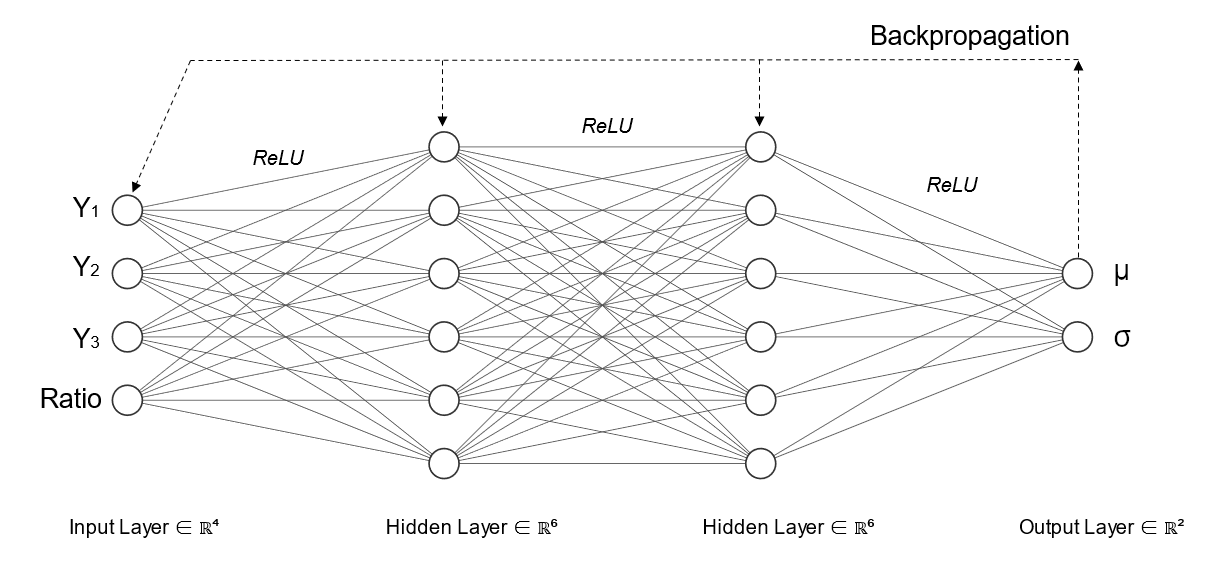
\includegraphics[scale=0.6]{BP.png}
    \caption{The BP Neural Network Structure}
\end{figure}

\subsection{Validation of the Model}

After training this BP neural network for $10^6$ iterations, the total MSE loss has been reduced to about $0.074$.

To validate the model's robustness, we divided the sample data into training set and testing set. The training set conrains 80\% of the data while the testing set contains 20\% of the data. We first train our model on the trainging set then test it on the testing set and compare the MSE loss of two sets. We randomly choose those two sets for 6 times and the result is shown in figure \ref{Train Set}. The difference between the training set and the testing set is about 10\% of the training set MSE loss, which is acceptable.

\begin{figure}[H]
    \centering
    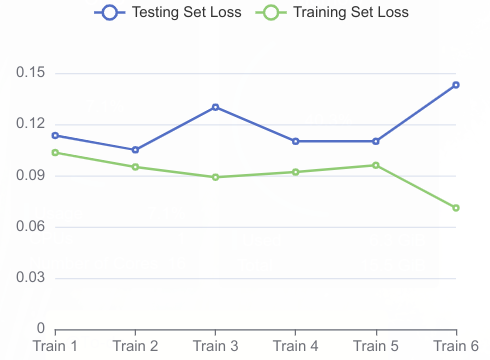
\includegraphics[scale=0.5]{trainingloss.png}
    \caption{MSE Loss of Training and Testing Set}
    \label{Train Set}
\end{figure}
